\documentclass{beamer}
\usepackage{amsmath,amssymb,amsfonts}
\usepackage{graphicx}
\usepackage{hyperref}
\usepackage{xcolor}

\title{CHAPTER - 3: Pair of Linear Equations in Two Variables}
\author{EE24BTECH11061 - Rohith Sai}
\date{January 23, 2025}

% Custom command for matrix representation
\newcommand{\myvec}[1]{\begin{bmatrix}#1\end{bmatrix}}

\begin{document}

% Title Page
\frame{\titlepage}

% Section for Exercise
\section*{Exercise 3.3}

% Question
\begin{frame}{Exercise 3.3 - Question}
\textbf{Solve the following pair of linear equations using LU decomposition:}
\begin{align*}
    x + y &= 14 \\
    x - y &= 4
\end{align*}
\end{frame}

% Solution Outline
\begin{frame}{Solution Outline}
\textbf{Steps to Solve:}
\begin{enumerate}
    \item Convert the given equations into matrix form.
    \item Apply LU decomposition to the coefficient matrix.
    \item Solve for intermediate variables (\(y_1, y_2\)) using forward substitution.
    \item Solve for unknowns (\(x, y\)) using backward substitution.
\end{enumerate}
\end{frame}

% Matrix Form
\begin{frame}{Step 1: Matrix Form}
\textbf{Matrix Representation:}
\begin{align*}
    \myvec{1 & 1 \\ 1 & -1}\myvec{x \\ y} &= \myvec{14 \\ 4} \\
    A\vec{x} &= \vec{b}
\end{align*}
Here:
\[
    A = \myvec{1 & 1 \\ 1 & -1}, \quad \vec{x} = \myvec{x \\ y}, \quad \vec{b} = \myvec{14 \\ 4}.
\]
\textbf{Objective:} Decompose $A$ into $L$ (Lower triangular) and $U$ (Upper triangular) matrices.
\end{frame}

% LU Decomposition Explanation
\begin{frame}{Step 2: LU Decomposition}
\textbf{LU Decomposition Steps:}
\begin{enumerate}
    \item Start with $A$ and initialize:
        \[
        L = \myvec{1 & 0 \\ 0 & 1}, \quad U = A
        \]
    \item For each row and column:
        \begin{align*}
        U_{k,j} &= A_{k,j} - \sum_{m=1}^{k-1} L_{k,m} \cdot U_{m,j}, \quad j \geq k, \\
        L_{i,k} &= \frac{1}{U_{k,k}} \left( A_{i,k} - \sum_{m=1}^{k-1} L_{i,m} \cdot U_{m,k} \right), \quad i > k.
        \end{align*}
\end{enumerate}
\end{frame}

% LU Decomposition Results
\begin{frame}{LU Decomposition Results}
\textbf{Decomposed Matrices:}
\[
L = \myvec{1 & 0 \\ 1 & 1}, \quad U = \myvec{1 & 1 \\ 0 & -2}.
\]
Verification:
\[
    A = L \cdot U
\]
\end{frame}

% Forward Substitution
\begin{frame}{Step 3: Forward Substitution}
\textbf{Solve for intermediate variables \(\vec{y}\):}
\[
L \cdot \vec{y} = \vec{b}.
\]
Substituting:
\[
\myvec{1 & 0 \\ 1 & 1}\myvec{y_1 \\ y_2} = \myvec{14 \\ 4}.
\]
Solution:
\begin{align*}
    y_1 &= 14, \\
    y_1 + y_2 &= 4 \implies y_2 = -10.
\end{align*}
\end{frame}

% Backward Substitution
\begin{frame}{Step 4: Backward Substitution}
\textbf{Solve for unknowns \(\vec{x}\):}
\[
U \cdot \vec{x} = \vec{y}.
\]
Substituting:
\[
\myvec{1 & 1 \\ 0 & -2}\myvec{x_1 \\ x_2} = \myvec{14 \\ -10}.
\]
Solution:
\begin{align*}
    x_2 &= 5, \\
    x_1 + x_2 &= 14 \implies x_1 = 9.
\end{align*}
\end{frame}

% Final Solution
\begin{frame}{Final Solution}
\textbf{The solution is:}
\[
x = 9, \quad y = 5.
\]
\end{frame}

% Graphical Representation
\begin{frame}{Graphical Representation}
\textbf{Graph of the equations:}
\begin{figure}
    \centering
    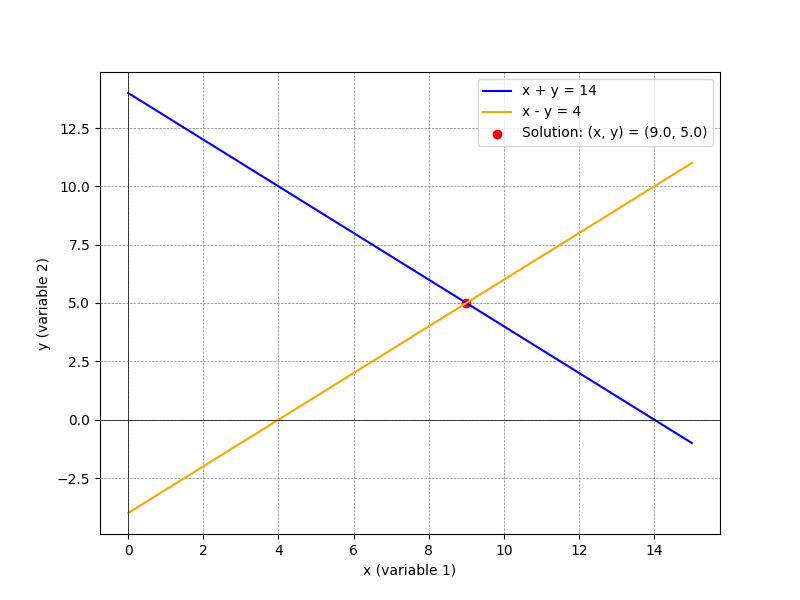
\includegraphics[width=0.8\textwidth]{figs/fig.png}
    \caption{Graphical Representation of the Solution}
\end{figure}
\end{frame}

% End of Document
\end{document}
